\section{Problem 3}
My implementation of K-means starts with randomly assign K centroids.
Then for each pixel I found the eucleidian distance between the centers
and the pixel. Then I add the pixel to the Kth minimum distance element
in order after dividing this with the number of points on this cluster to
get the new center. The code can be found in problem3.m. It has as an
argument the number of clusters it should produce. It returns the number
of clusters with at least a pixel in.
\begin{figure}[ht] 
  \begin{subfigure}[b]{0.5\linewidth}
    \centering
    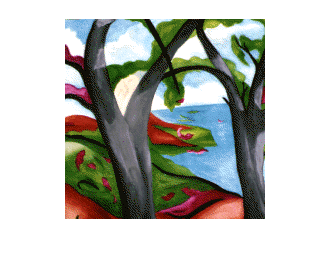
\includegraphics[width=0.75\linewidth]{figures/initial.png}
    \caption{Initial image} 
    \vspace{4ex}
  \end{subfigure}%% 
  \begin{subfigure}[b]{0.5\linewidth}
    \centering
    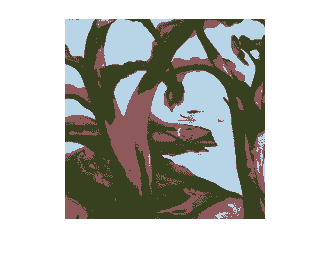
\includegraphics[width=0.75\linewidth]{figures/kmeans3.png} 
    \caption{K=3 clusters}
    \vspace{4ex}
  \end{subfigure} 
  \begin{subfigure}[b]{0.5\linewidth}
    \centering
    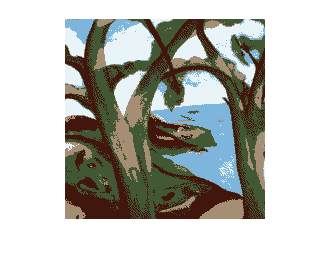
\includegraphics[width=0.75\linewidth]{figures/kmeans5.png}
    \caption{K=5 clusters} 
  \end{subfigure}%%
  \begin{subfigure}[b]{0.5\linewidth}
    \centering
    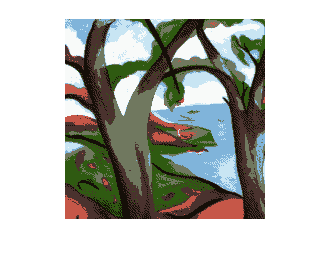
\includegraphics[width=0.75\linewidth]{figures/kmeans8.png} 
    \caption{K=8 clusters} 
  \end{subfigure} 
  \caption{Illustration of various K-means clustering}
\end{figure}
